\documentclass[Eubank_pk_ethnic_sorting.tex]{subfiles}

\begin{document}

Observational studies pointing to the superior performance of private schools are not the only reason that education reform advocates have voiced excitement about the potential of private school growth; private schools also operate in fundamentally different ways from government schools. For that reason, it is important to examine not only whether the government-private performance differential varies with caste heterogeneity, but also whether other factors some suspect explain school differences can be ruled out as alternate explanations.


\subsection{Differences in Teacher Incentives}\label{incentives}

Advocates of private schools argue that not only are observational studies able to control for many factors, but there is also evidence to explain \emph{why} private schools outperform government schools. In particular, they point out that private schools appear to address the biggest problem in government schools: low effort. High absenteeism and low accountability in government schools has been well documented \citep{Muralidharan:2008tb, Chaudhury:2006vp}, but appears less prevalent in private schools. The reason, many argue, is that in private schools good teachers are better paid, and poor teachers are let go. This line of reasoning is also buoyed by a growing body of literature that suggests that what matters for success is not the availability of educational ``inputs'' (like qualified, well paid teachers or good facilities), but incentive schemes that reward effort on the behalf of teachers \citep{Hanushek:1997tt,Hanushek:2003hz,Banerjee:2007wx}.

The conclusion of the LEAPS survey authors (full disclosure: this author was a research assistant on the LEAPS project, though not an author) is that this is the case in Pakistan. Private schools deliver better educational outcomes despite hiring only secondary-educated local women with no training and providing them with relatively low wages because private schools incentize good teaching by paying good teachers more, improving effort. This differentiates them from government schools, which offer salaries which are higher but unresponsive to performance. As a result, the authors argue, government school teachers exert less effort. This is illustrated in Figure~\ref{payandabsenteeism} which appears in the original LEAPS report \citep{Andrabi:2007we}. It shows that while frequently absent private school teachers are paid less, absent government school teachers are actually paid \emph{more}. And where private school teachers with high score students are paid more, no such relationship exists for government teachers.

DROP FIGURE

% \begin{figure}[htb]
% 	\begin{center}
% 	\caption{Teacher Performance and Compensation}\label{payandabsenteeism}
% 	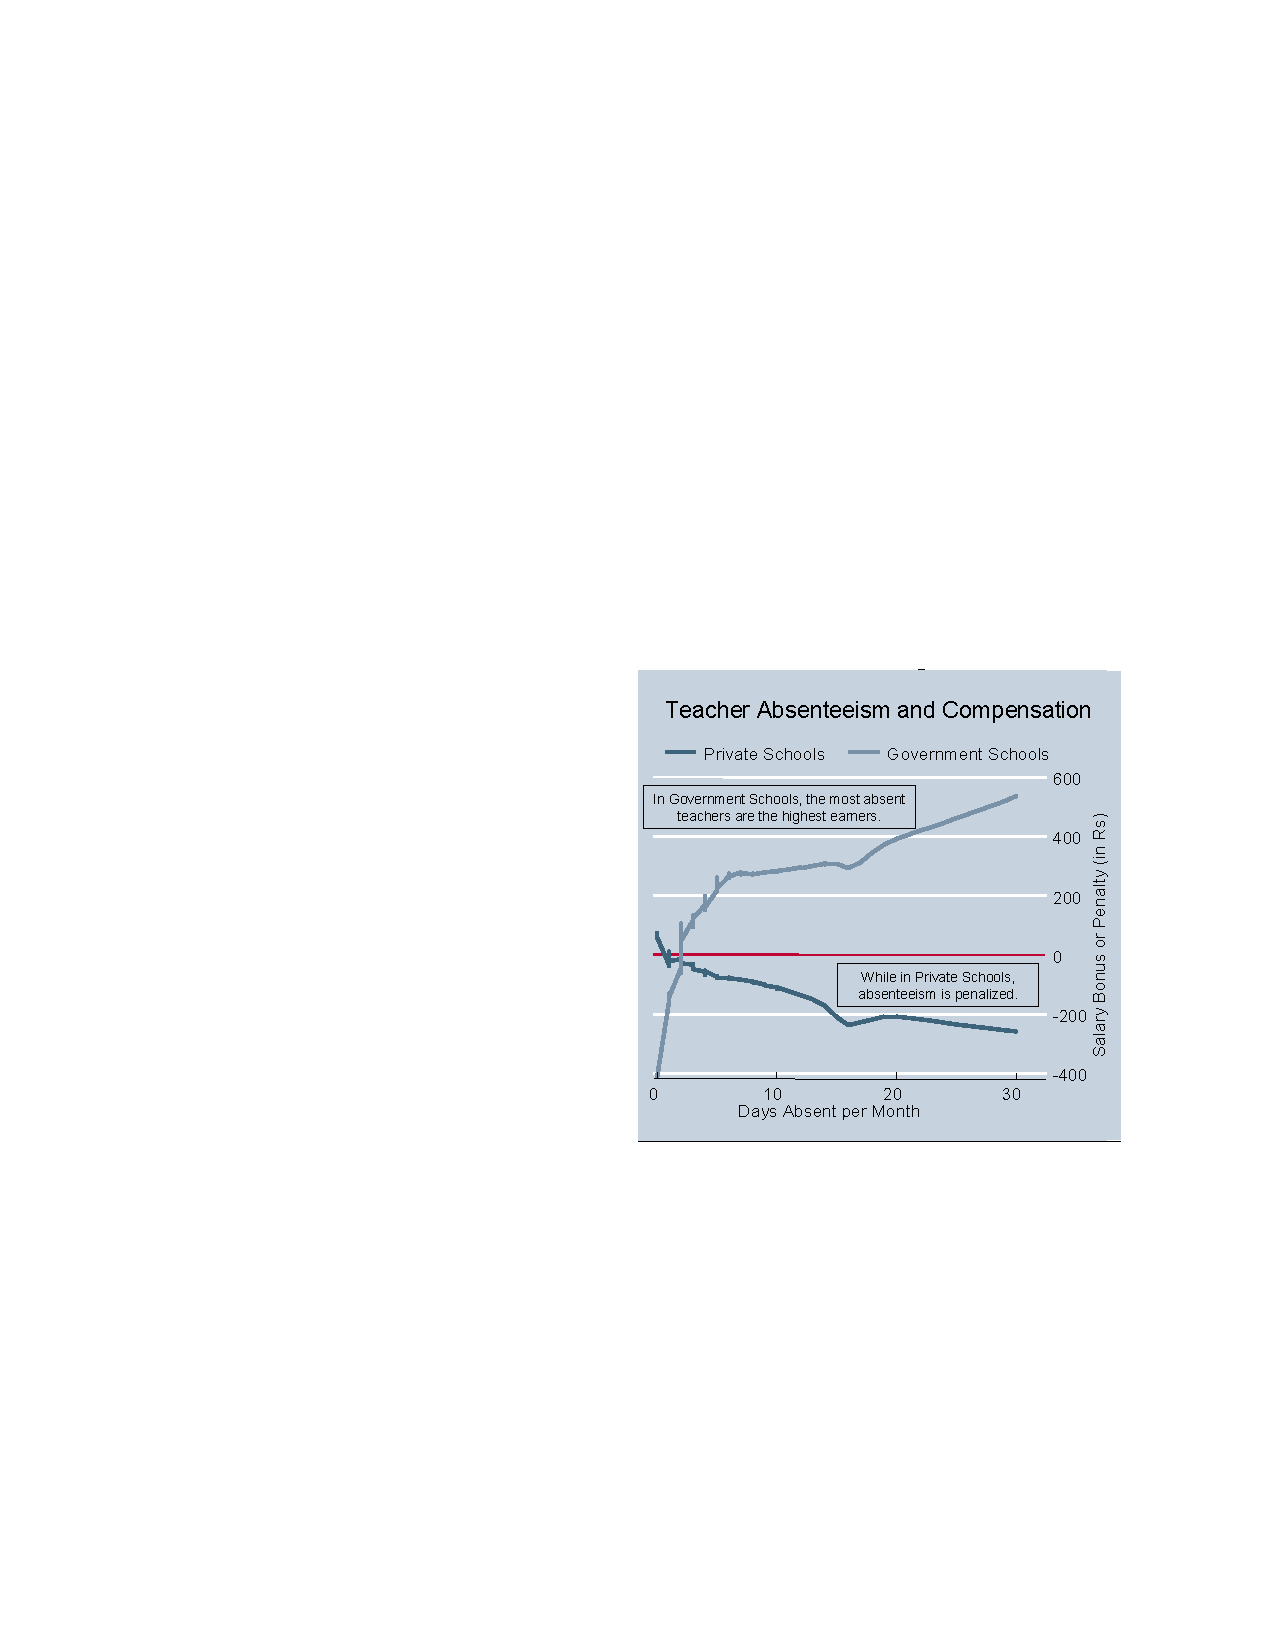
\includegraphics[scale=0.82]{../results/absenteeism_and_pay.pdf} 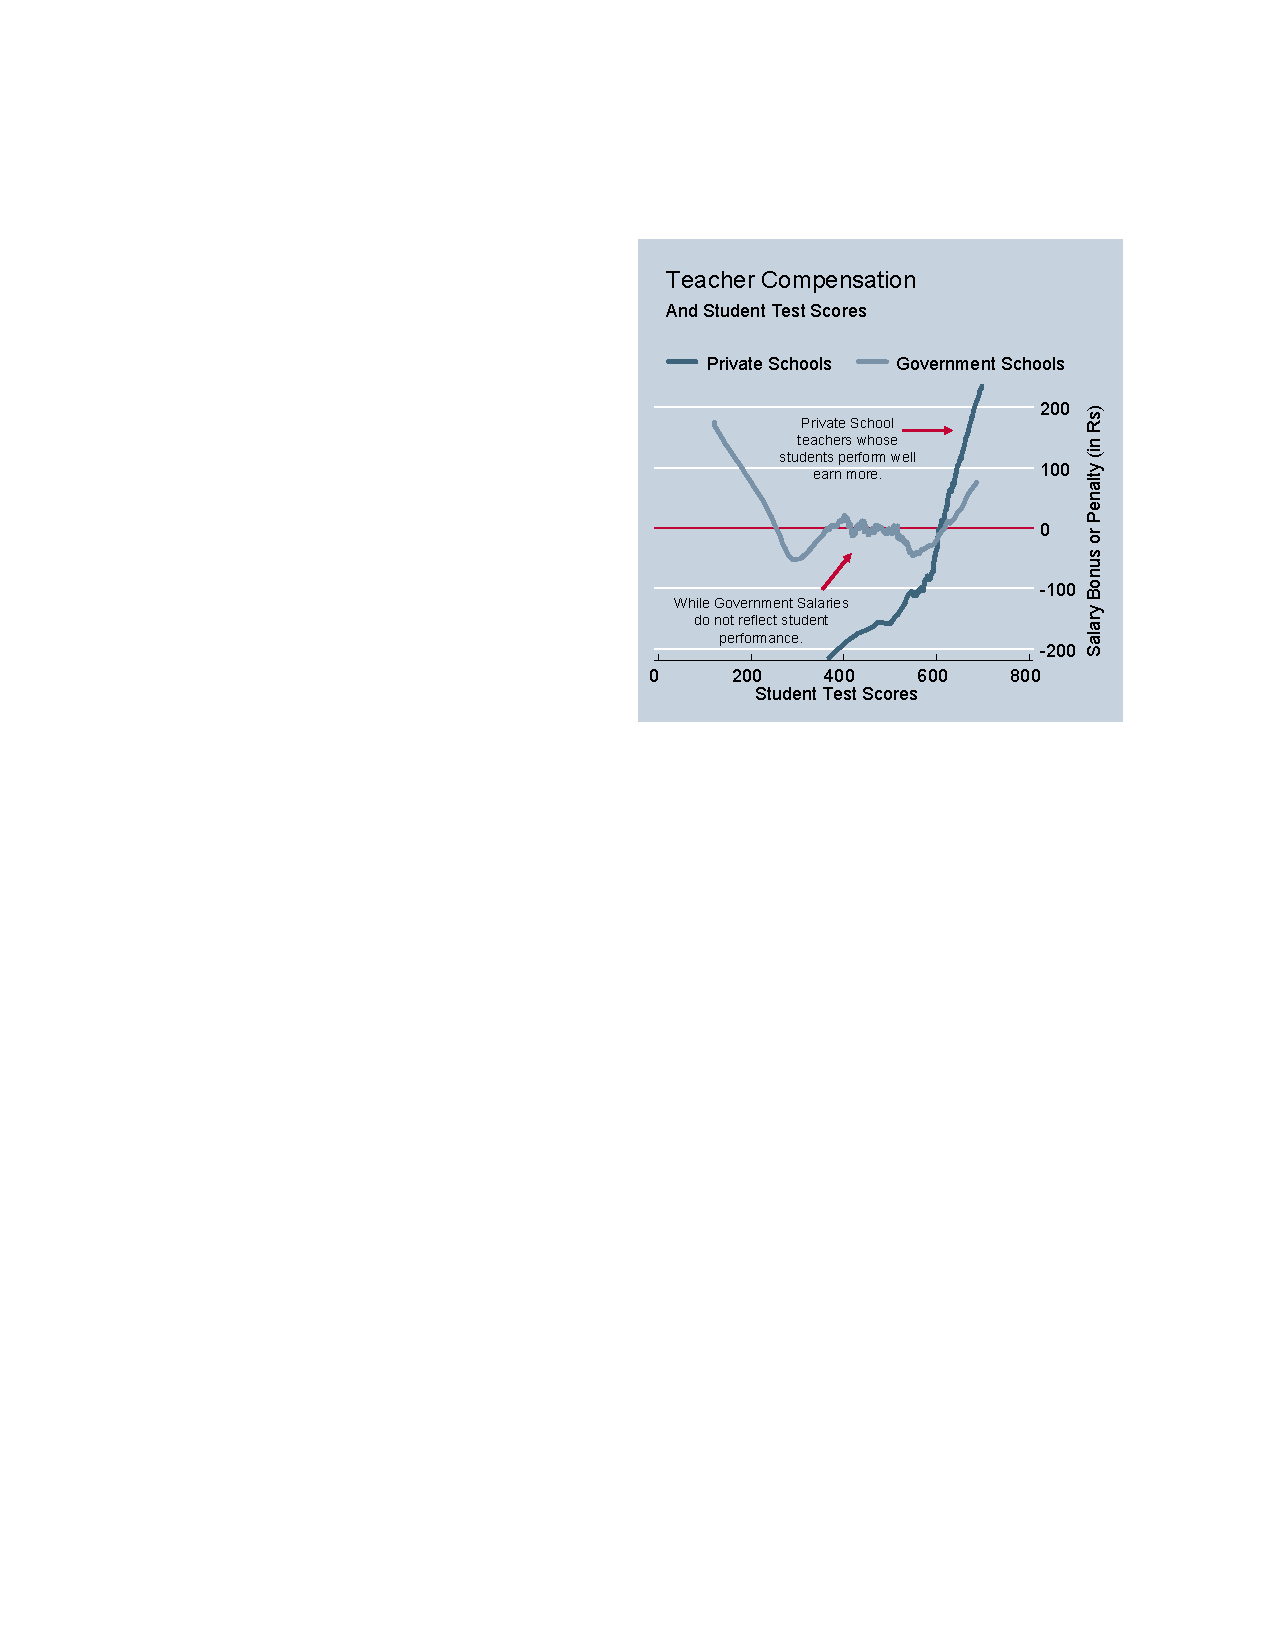
\includegraphics[scale=0.8]{../results/compensation_scores.pdf}\\
% 	\emph{Source: \cite{Andrabi:2007we}, pages 72, 74. Salary bonus or penalty is the degree to which salary differences from predicted values independent of absenteeism or test scores.}
% 	\end{center}
% \end{figure}

Table~\ref{teachercompensation} below recreates the analyses underlying the two plots in Figure~\ref{payandabsenteeism} with two adjustments: first, rather than measuring performance using average test scores (in levels), more rigorous teacher ``value-added'' scores (Specification~\ref{teacherspecification}) are employed to measure teacher contributions to learning; second, a village fractionalization measure is included in all results as an interaction term. If it is the case that differences in incentive schemes are driving test score convergence, then we should see (a) the private-school salary penalty for absenteeism decline in fractionalization, and (b) the compensation premium (compensation above what is otherwise predicted) for performance decline. As shown in the table, however, the absenteeism penalty actually \emph{increases} in fractionalization (which under the incentive story should result in \emph{increased} private school scores), and no relationship exists between performance and compensation. In sum, there is no relationship between fractionalization and how government teachers are compensated.


\begin{table}[htbp]\centering
\def\sym#1{\ifmmode^{#1}\else\(^{#1}\)\fi}
\caption{Village Fractionalization and Teacher Compensation\label{teachercompensation}}
\begin{tabular}{l*{4}{c}}
\toprule
                &\multicolumn{2}{c}{Private Teachers}&\multicolumn{2}{c}{Government Teachers}\\\cmidrule(lr){2-3}\cmidrule(lr){4-5}
                &\multicolumn{1}{c}{(1)}&\multicolumn{1}{c}{(2)}&\multicolumn{1}{c}{(3)}&\multicolumn{1}{c}{(4)}\\
                &\multicolumn{1}{c}{Log Salary}&\multicolumn{1}{c}{Log Salary}&\multicolumn{1}{c}{Log Salary}&\multicolumn{1}{c}{Log Salary}\\
\midrule
Days Absent Last Month&    0.041** &  -0.0068   &   0.0017   &   0.0041***\\
                &   (2.00)   &  (-0.85)   &   (0.40)   &   (2.79)   \\
Biraderi Fractionalization&     0.24   &     0.21   &   -0.085   &   -0.050   \\
                &   (1.18)   &   (0.78)   &  (-1.47)   &  (-0.74)   \\
Days Absent * Fractionalization&   -0.063** &            &   0.0050   &            \\
                &  (-2.05)   &            &   (0.77)   &            \\
Gender          &    -0.32***&    -0.27** &   -0.012   &   0.0095   \\
                &  (-3.78)   &  (-2.17)   &  (-0.72)   &   (0.54)   \\
Age of teacher  &   0.0053   &    0.023** &    0.021***&    0.018***\\
                &   (1.21)   &   (2.54)   &  (12.18)   &  (14.48)   \\
Average Value Added Score&            &     0.22   &            &   -0.033   \\
                &            &   (0.48)   &            &  (-0.48)   \\
Value-Added * Fractionalization&            &    -0.47   &            &   -0.020   \\
                &            &  (-0.67)   &            &  (-0.22)   \\
Constant        &     7.07***&     8.02***&     7.51***&     7.60***\\
                &  (29.09)   &  (20.15)   &  (47.83)   &  (61.24)   \\
District Fixed Effects&      Yes   &      Yes   &      Yes   &      Yes   \\
\midrule
Observations    &      619   &      154   &     1302   &      618   \\
\bottomrule
\multicolumn{5}{l}{\footnotesize \specialcell{Controls for Experience and Teacher Education excluded from table.\\Robust t-statistics clustered at the village level in parenthesis}}\\
\multicolumn{5}{l}{\footnotesize * p<0.10, ** p<0.05, *** p<0.01}\\
\end{tabular}
\end{table}



\subsection{Differences in School Inputs}

A second potential explanation for variation in the government-private school performance differential is that the availability of school resources varies with village caste heterogeneity. To test this, this paper examines the relationship between village fragmentation and different school inputs.

Table~\ref{privateteachers} presents a series of school-level results in which measures of school- and teacher-quality in private schools are regressed against village fractionalization and a number of controls. The table shows that there is little or no evidence that -- at least in terms of visible inputs -- differences in inputs can explain the decline in private school performance in fractionalized villages. If anything, private school teachers appear to be slightly \emph{better} educated in fractionalized villages.

\begin{sidewaystable}[htbp]\centering
\def\sym#1{\ifmmode^{#1}\else\(^{#1}\)\fi}
\caption{Private Teacher Characteristics and Village Fractionalization\label{privateteachers}}
\begin{tabular}{l*{6}{c}}
\toprule
                &\multicolumn{1}{c}{(1)}&\multicolumn{1}{c}{(2)}&\multicolumn{1}{c}{(3)}&\multicolumn{1}{c}{(4)}&\multicolumn{1}{c}{(5)}&\multicolumn{1}{c}{(6)}\\
                &\multicolumn{1}{c}{\specialcellc{Days Absent \\ Last Month}}&\multicolumn{1}{c}{Female}&\multicolumn{1}{c}{\specialcellc{Local \\ Teacher}}&\multicolumn{1}{c}{\specialcellc{More than Grade \\ School Educ}}&\multicolumn{1}{c}{\specialcellc{Teacher's \\ English Score}}&\multicolumn{1}{c}{\specialcellc{Basic School \\ Facility Index}}\\
\midrule
Biraderi Fractionalization&    -0.13   &    -0.15   &     0.21   &     0.11   &     0.30   &     0.45   \\
                &   (0.34)   &  (0.096)   &   (0.16)   &  (0.080)   &   (0.19)   &   (0.68)   \\
\specialcell{Median Village \\ Expenditures}&0.0000047   & 0.000032   &0.0000038   &0.0000096   & 0.000038   &-0.000081   \\
                &(0.000061)   &(0.000021)   &(0.000019)   &(0.000016)   &(0.000024)   &(0.000096)   \\
\specialcell{Log Number \\ of Households}&    0.061   &  -0.0067   &   -0.072*  &   -0.030   &    0.038   &    -0.24*  \\
                &   (0.10)   &  (0.022)   &  (0.039)   &  (0.020)   &  (0.033)   &   (0.13)   \\
District Fixed Effects&      Yes   &      Yes   &      Yes   &      Yes   &      Yes   &      Yes   \\
\midrule
Observations    &     4667   &     4675   &     4670   &     4675   &     1041   &      295   \\
\bottomrule
\multicolumn{7}{l}{\footnotesize Standard errors in parentheses}\\
\multicolumn{7}{l}{\footnotesize * \(p<0.10\), ** \(p<0.05\), *** \(p<0.01\)}\\
\multicolumn{7}{l}{\footnotesize All results clustered at the village level.}\\
\end{tabular}
\end{sidewaystable}


Table~\ref{governmentteachers} repeats this exercise for government schools. It should be noted that government schools in Pakistan are administered at the state level, and are thus relatively insulated from village politics, making any such differences unlikely. Nevertheless, results are presented for thoroughness. These results show no difference in school inputs across villages.

\begin{sidewaystable}[htbp]\centering
\def\sym#1{\ifmmode^{#1}\else\(^{#1}\)\fi}
\caption{Government Teacher Characteristics and Village Fractionalization\label{governmentteachers}}
\begin{tabular}{l*{6}{c}}
\toprule
                &\multicolumn{1}{c}{(1)}&\multicolumn{1}{c}{(2)}&\multicolumn{1}{c}{(3)}&\multicolumn{1}{c}{(4)}&\multicolumn{1}{c}{(5)}&\multicolumn{1}{c}{(6)}\\
                &\multicolumn{1}{c}{Days Absent Last Month}&\multicolumn{1}{c}{Female}&\multicolumn{1}{c}{From Village}&\multicolumn{1}{c}{\specialcellc{Teacher English \ Exam Score}}&\multicolumn{1}{c}{\specialcellc{More than Grade \ School Education}}&\multicolumn{1}{c}{\specialcellc{Basic School \\ Facility Index}}\\
\midrule
Biraderi Fractionalization&    -0.67   &    0.048   &     0.13   &     0.19   &    0.092   &     0.45   \\
                &   (0.56)   &   (0.13)   &   (0.19)   &   (0.19)   &   (0.11)   &   (0.68)   \\
\specialcell{Median Village \\\\ Expenditures}& 0.000089   & 0.000031   &-0.000016   & 0.000029   & 0.000016   &-0.000081   \\
                &(0.000077)   &(0.000027)   &(0.000025)   &(0.000022)   &(0.000015)   &(0.000096)   \\
\specialcell{Log Number \\\\ of Households}&   -0.068   &   -0.033   &   -0.082   &   -0.015   &   -0.034** &    -0.24*  \\
                &  (0.096)   &  (0.024)   &  (0.050)   &  (0.036)   &  (0.015)   &   (0.13)   \\
District Fixed Effects&      Yes   &      Yes   &      Yes   &      Yes   &      Yes   &      Yes   \\
\midrule
Observations    &     1335   &     1337   &     1335   &      990   &     1337   &      295   \\
\bottomrule
\multicolumn{7}{l}{\footnotesize Standard errors in parentheses}\\
\multicolumn{7}{l}{\footnotesize * p<0.10, ** p<0.05, *** p<0.01}\\
\end{tabular}
\end{sidewaystable}




\end{document}
